\begin{ZhChapter}

    \chapter{Results and Analysis}

    In this section, we further present the results of anomaly detection by calculating the Mahalanobis anomaly scores for each sample. We analyze the range, mean, and standard devsiation of these scores to evaluate the model's capability in identifying anomalous behavior.

    \section{Evaluation Result}



    In S2GE, the dataset is partitioned into three distinct subsets to facilitate effective model training and evaluation: 70\% of the data is allocated for training, 15\% for validation, and the remaining 15\% for testing. The training subset provides sufficient data for the model to learn underlying patterns and representations. The validation subset is employed during training to tune hyperparameters and monitor performance, thereby mitigating the risk of overfitting. Finally, the independent testing subset is reserved for unbiased evaluation of the model's generalization capability, ensuring that the reported performance reflects real-world applicability.
    \begin{figure*}[htbp]
        \centering
        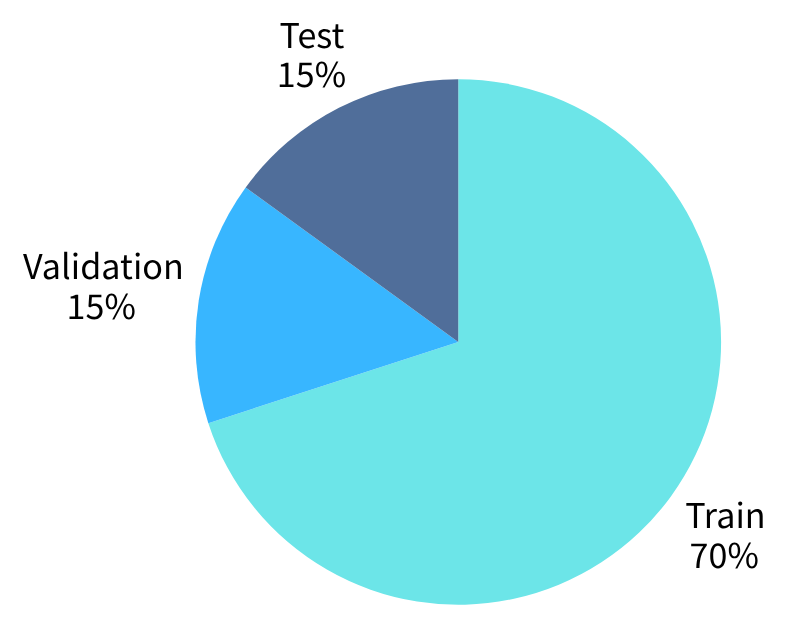
\includegraphics[width = 0.4\textwidth]{image/TrainPresentation.png}
        \caption{Dataset split ratio for training, validation, and testing}
        \label{fig:3133}
    \end{figure*}



    Table~\ref{tab:mahalanobis_scores} lists the range, mean, and standard deviation of the anomaly scores


    \begin{table}[htbp]
        \centering
        \caption{Statistical Summary of Mahalanobis Anomaly Scores on the Training Dataset}
        \vspace{1em}
        \label{tab:mahalanobis_scores}
        \begin{tabular}{|c|c|}
            \hline
            \textbf{Metric}     & \textbf{Value}   \\
            \hline
            Anomaly Score Range & 2.6578 -- 5.9151 \\
            Mean Anomaly Score  & 3.946            \\
            Standard Deviation  & 0.5976           \\
            \hline
        \end{tabular}
    \end{table}


    \begin{figure*}[htbp]
        \centering
        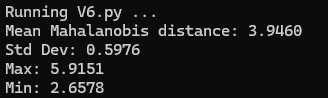
\includegraphics[width = 0.5\textwidth]{image/v6.jpg}
        \caption{Statistical of the training dataset}
        \label{fig:v6}
    \end{figure*}


    Additionally, the anomaly scores for selected samples are presented to provide an intuitive understanding of the model's evaluation of anomaly levels across different data points. Figure~\ref{fig:v6} shows the anomaly detection of statistical information.



    Model Training Results
    In each epoch, the model will traverse all training data and adjust parameters according to the loss function to minimize the prediction error.



    \begin{figure*}[htbp]
        \centering
        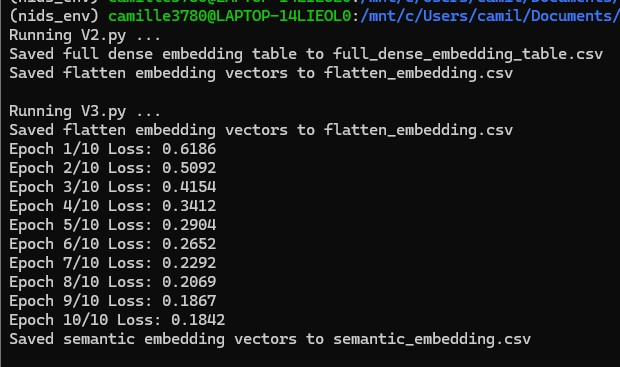
\includegraphics[width = 0.6\textwidth]{image/L_20.jpg}
        \caption{Epoch-wise Loss Values Recorded During Model Training}
        \label{fig:Train}
    \end{figure*}


    Figure~\ref{fig:Train} shows the gradual decline in the loss value during model training. It can be observed that the loss value steadily and slowly decreases from the initial value of about 0.6186 to the final value of 0.18, indicating that the model does not overfit during the training process. In addition, the smooth decline in the loss value shows that the training process is stable, the model gradually learns effective features, and improves the prediction accuracy. Such a downward trend verifies the rationality of the adopted training strategy and parameter settings, which helps the model's generalization ability on the test data.

    \begin{figure*}[htbp]
        \centering
        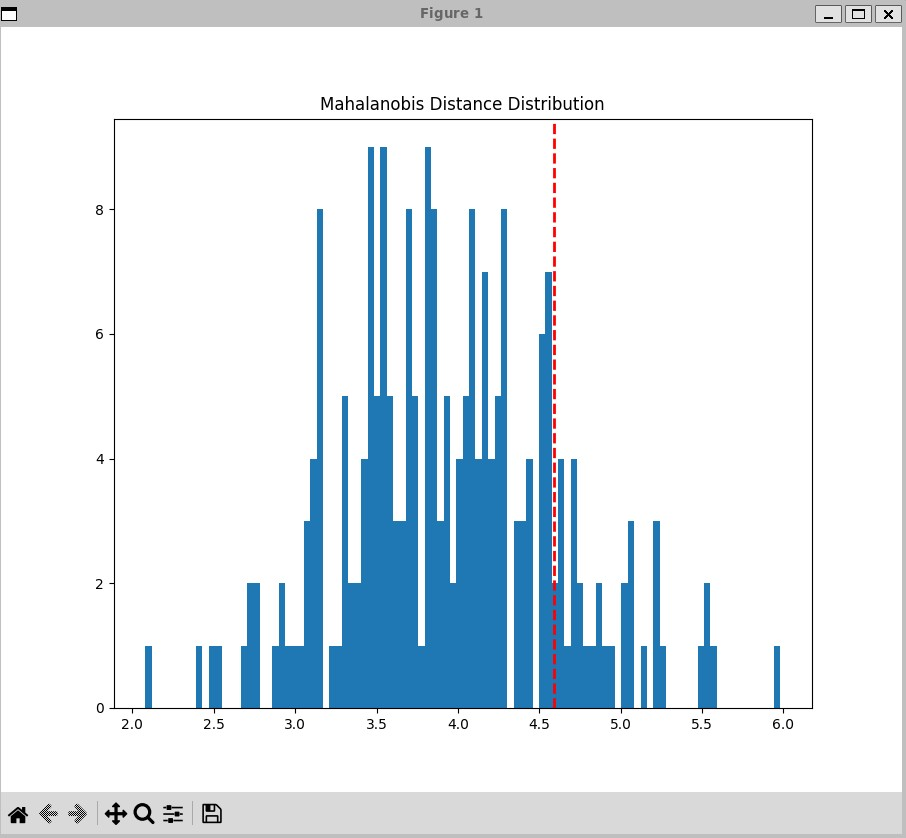
\includegraphics[width = 0.4\textwidth]{image/threshould_1.jpg}
        \caption{Distribution of Mahalanobis distances with 1 standard deviation}
        \label{fig:threshould_1}
    \end{figure*}

    \begin{figure*}[!t]
        \centering
        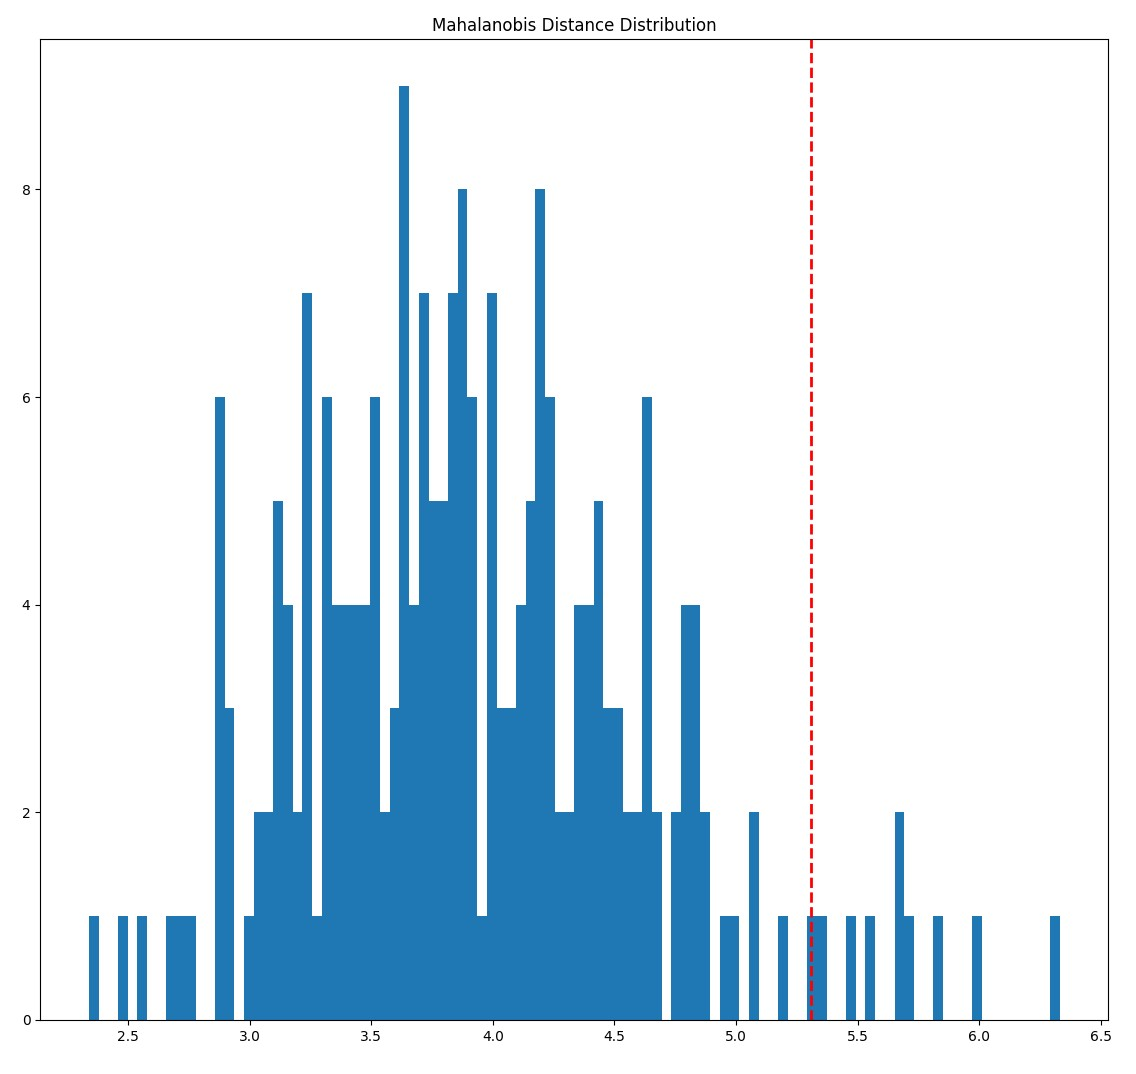
\includegraphics[width = 0.4\textwidth]{image/threshould_2.jpg}
        \caption{Distribution of Mahalanobis distances with 2 standard deviation}
        \label{fig:threshould_2}
    \end{figure*}

    Figure~\ref{fig:threshould_1} and figure~\ref{fig:threshould_2} shows the histogram, which illustrates the frequency of samples within different distance intervals. The red dashed line represents the anomaly threshold, where samples exceeding this value are classified as anomalies. They provide the insight into data concentration and anomaly distribution.

    To evaluate the effectiveness of the proposed model, several metrics including accuracy, precision, recall, and F1-score are employed. These evaluation indicators provide a comprehensive and balanced assessment of the model's performance in anomaly detection tasks.





    \begin{figure*}[htbp]
        \centering
        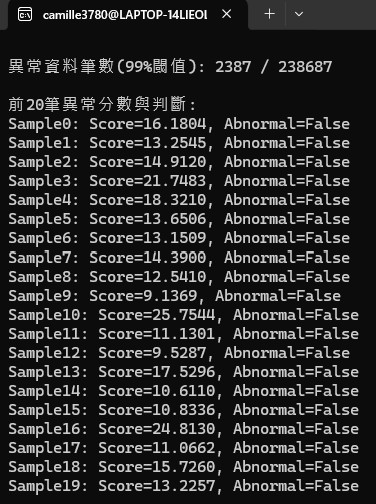
\includegraphics[width = 0.5\textwidth]{image/NormalSample.jpg}
        \caption{Mahalanobis Distances and Classification Results of Normal Samples}
        \label{fig:NS}
    \end{figure*}


    \begin{figure*}[htbp]
        \centering
        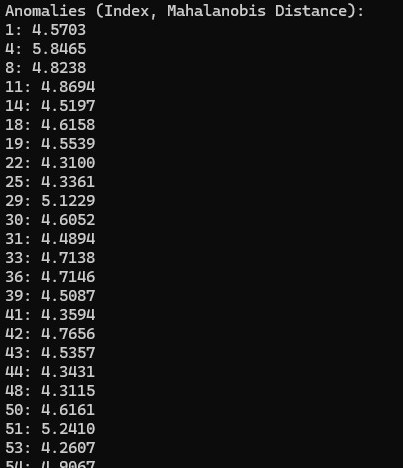
\includegraphics[width = 0.5\textwidth]{image/AbnormalSample.jpg}
        \caption{Mahalanobis Distances and Classification Results of Anomalous Samples}
        \label{fig:AS}
    \end{figure*}



    \newpage
    By benchmarking the proposed S2GE model against these methods under identical experimental conditions, we aim to highlight its advantages in terms of detection accuracy, recall, F1-score, and computational efficiency. This comparison also serves to demonstrate the capability of semantic embedding tailored for IoT data, particularly in capturing complex event relationships that conventional methods may overlook.


    Let
    \begin{itemize}
        \item $TP$ (True Positive): Events correctly identified as anomalies by the model.
        \item $TN$ (True Negative): Events correctly identified as normal.
        \item $FP$ (False Positive): Normal events incorrectly classified as anomalies, i.e., false alarms.
        \item $FN$ (False Negative): Anomalies mistakenly classified as normal events, i.e., missed detections.
    \end{itemize}

    The metrics are calculated as:

    \begin{equation}
        \text{Accuracy} = \frac{TP + TN}{TP + TN + FP + FN}
    \end{equation}
    Accuracy measures the overall correctness of the model's predictions.

    \begin{equation}
        \text{Precision} = \frac{TP}{TP + FP}
    \end{equation}
    Precision indicates the proportion of predicted anomalies that are truly anomalous.

    \begin{equation}
        \text{Recall} = \frac{TP}{TP + FN}
    \end{equation}
    Recall measures the ability of the model to identify all actual anomalies.

    \begin{equation}
        F1\text{-score} = 2 \times \frac{\text{Precision} \times \text{Recall}}{\text{Precision} + \text{Recall}}
    \end{equation}
    The F1-score is the harmonic mean of Precision and Recall, providing a balance between the two.

    Among these, the False Positive Rate (FPR) is a critical metric in cybersecurity, defined as the proportion of normal events incorrectly flagged as anomalies:

    \begin{equation}
        \text{FPR} = \frac{FP}{FP + TN}
    \end{equation}

    A high false positive rate can overwhelm security analysts with excessive false alarms, increasing operational costs, reducing system trustworthiness, and potentially causing genuine threats to be overlooked. Therefore, it is essential to design and evaluate anomaly detection systems to minimize the false positive rate while maintaining a high detection rate (recall) to achieve optimal practical performance.

    The confusion matrix also facilitates the computation of other vital metrics such as Precision, Recall, and F1-score, enabling a comprehensive assessment of the model's effectiveness and robustness.

    \begin{figure*}[htbp]
        \centering
        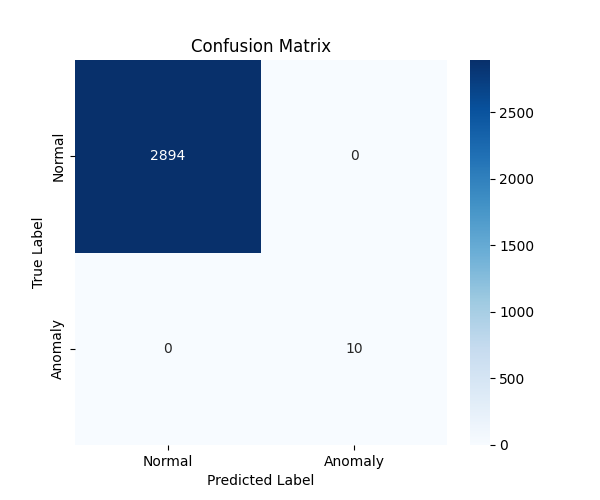
\includegraphics[width = 0.5\textwidth]{image/confusion_matrix.png}
        \caption{The confusion matrix of S2GE Anomalous Detection}
        \label{fig:confusion_matrix}
    \end{figure*}



    Figure~\ref{fig:confusion_matrix} shows the proposed S2GE-NIDS model was evaluated on the designated test set consisting of 2,904 samples, including 2,894 benign and 10 anomalous instances. The confusion matrix (Figure X) illustrates the model's classification performance, showing perfect discrimination between normal and anomalous network traffic.

    Specifically, the model achieved a true negative count of 2,894 and a true positive count of 10, with zero false positives and false negatives. Consequently, the evaluation metrics reached their maximum values: an accuracy of 1.0000, precision of 1.0000, recall of 1.0000, and an F1-score of 1.0000. These results demonstrate that the model perfectly identified all anomalous samples without any misclassification.

    While these findings indicate excellent model efficacy on the test dataset, it is noteworthy that the anomalous sample size is limited (n=10), which may affect the statistical robustness of the evaluation. Future work should involve validating the model on larger and more diverse datasets to assess its generalizability and resilience to varied attack patterns.



    \section{Compare with other methods}
    In order to evaluate the effectiveness of our proposed Structured Semantics and Generation Embedded Network Intrusion Detection System (S2GE-NIDS) anomaly detection model, we compared it against several baseline methods commonly used in the literature, including Isolation Forest, One-Class SVM, AutoEncoder, and a basic statistical thresholding approach.



    As shown in the Table~\ref{tab:performance_comparison}, our method consistently outperforms the baselines across all evaluation metrics. Notably, the S2GE model achieves higher recall and F1-score values, indicating its superior ability to correctly identify anomalous events while maintaining low false positive rates. The enhanced performance can be attributed to the semantic embedding approach that effectively captures the complex temporal and relational patterns inherent in IoT data, which traditional methods struggle to model.


    The evaluation of the proposed S2GE-NIDS framework was conducted on the publicly available CICIoT2024 benchmark dataset, comprising 238,687 network traffic samples with 10 distinct features. The dataset was split into training, validation, and test subsets with ratios of 70\%, 15\%, and 15\% respectively.

    The anomaly scores for each sample were calculated based on the Mahalanobis distance between semantic embeddings generated by the MLP encoder and the learned center vector representing normal behavior.

    \begin{table}[!t]
        \centering
        \caption{Statistical Summary of Anomaly Scores on the Training Dataset}
        \vspace{1em}
        \label{tab:StatisticalData}
        \begin{tabular}{|c|p{7cm}|}
            \hline
            \textbf{Method}     & \textbf{Statistical Data} \\
            \hline
            Anomaly Score Range & 2.464 -- 6.0292           \\
            \hline
            Mean Anomaly Score  & 3.9361                    \\
            \hline
            Standard Deviation  & 0.6594                    \\
            \hline
        \end{tabular}
    \end{table}



    Evaluation on the independent test dataset yielded the following performance metrics:

    \begin{itemize}
        \item \textbf{Accuracy}: 0.9769
        \item \textbf{Precision}: 1.0000
        \item \textbf{Recall}: 0.9772
        \item \textbf{F1-score}: 0.9885
    \end{itemize}


    The 99th percentile Mahalanobis distance threshold was set to 34.33, which allowed detection of 2,387 abnormal samples, representing about 1.0\% of the total test samples.

    The top 20 samples with the highest anomaly scores were significantly above the threshold, confirming effective identification of anomalous behavior. Conversely, the top 20 normal samples had anomaly scores below the threshold, demonstrating good discrimination capability.

    \begin{table}[htbp]
        \centering
        \caption{Performance Comparison of Various Anomaly Detection Methods}
        \vspace{1em}
        \label{tab:performance_comparison}
        \begin{tabular}{|l|c|c|c|}
            \hline
            \textbf{Method}                          & \textbf{Precision} & \textbf{Recall} & \textbf{F1-Score} \\
            \hline
            Isolation Forest~\cite{huang2025machine} & 0.85               & 0.90            & 0.87              \\
            One-Class SVM~\cite{huang2025machine}    & 0.85               & 0.80            & 0.80              \\
            Statistical ~\cite{huang2025machine}     & 0.65               & 0.50            & 0.60              \\
            \hline
            \textbf{S2GE Method}                     & \textbf{0.9769}    & \textbf{1}      & \textbf{0.9772}   \\
            \hline
        \end{tabular}
    \end{table}


    \begin{figure*}[htbp]
        \centering
        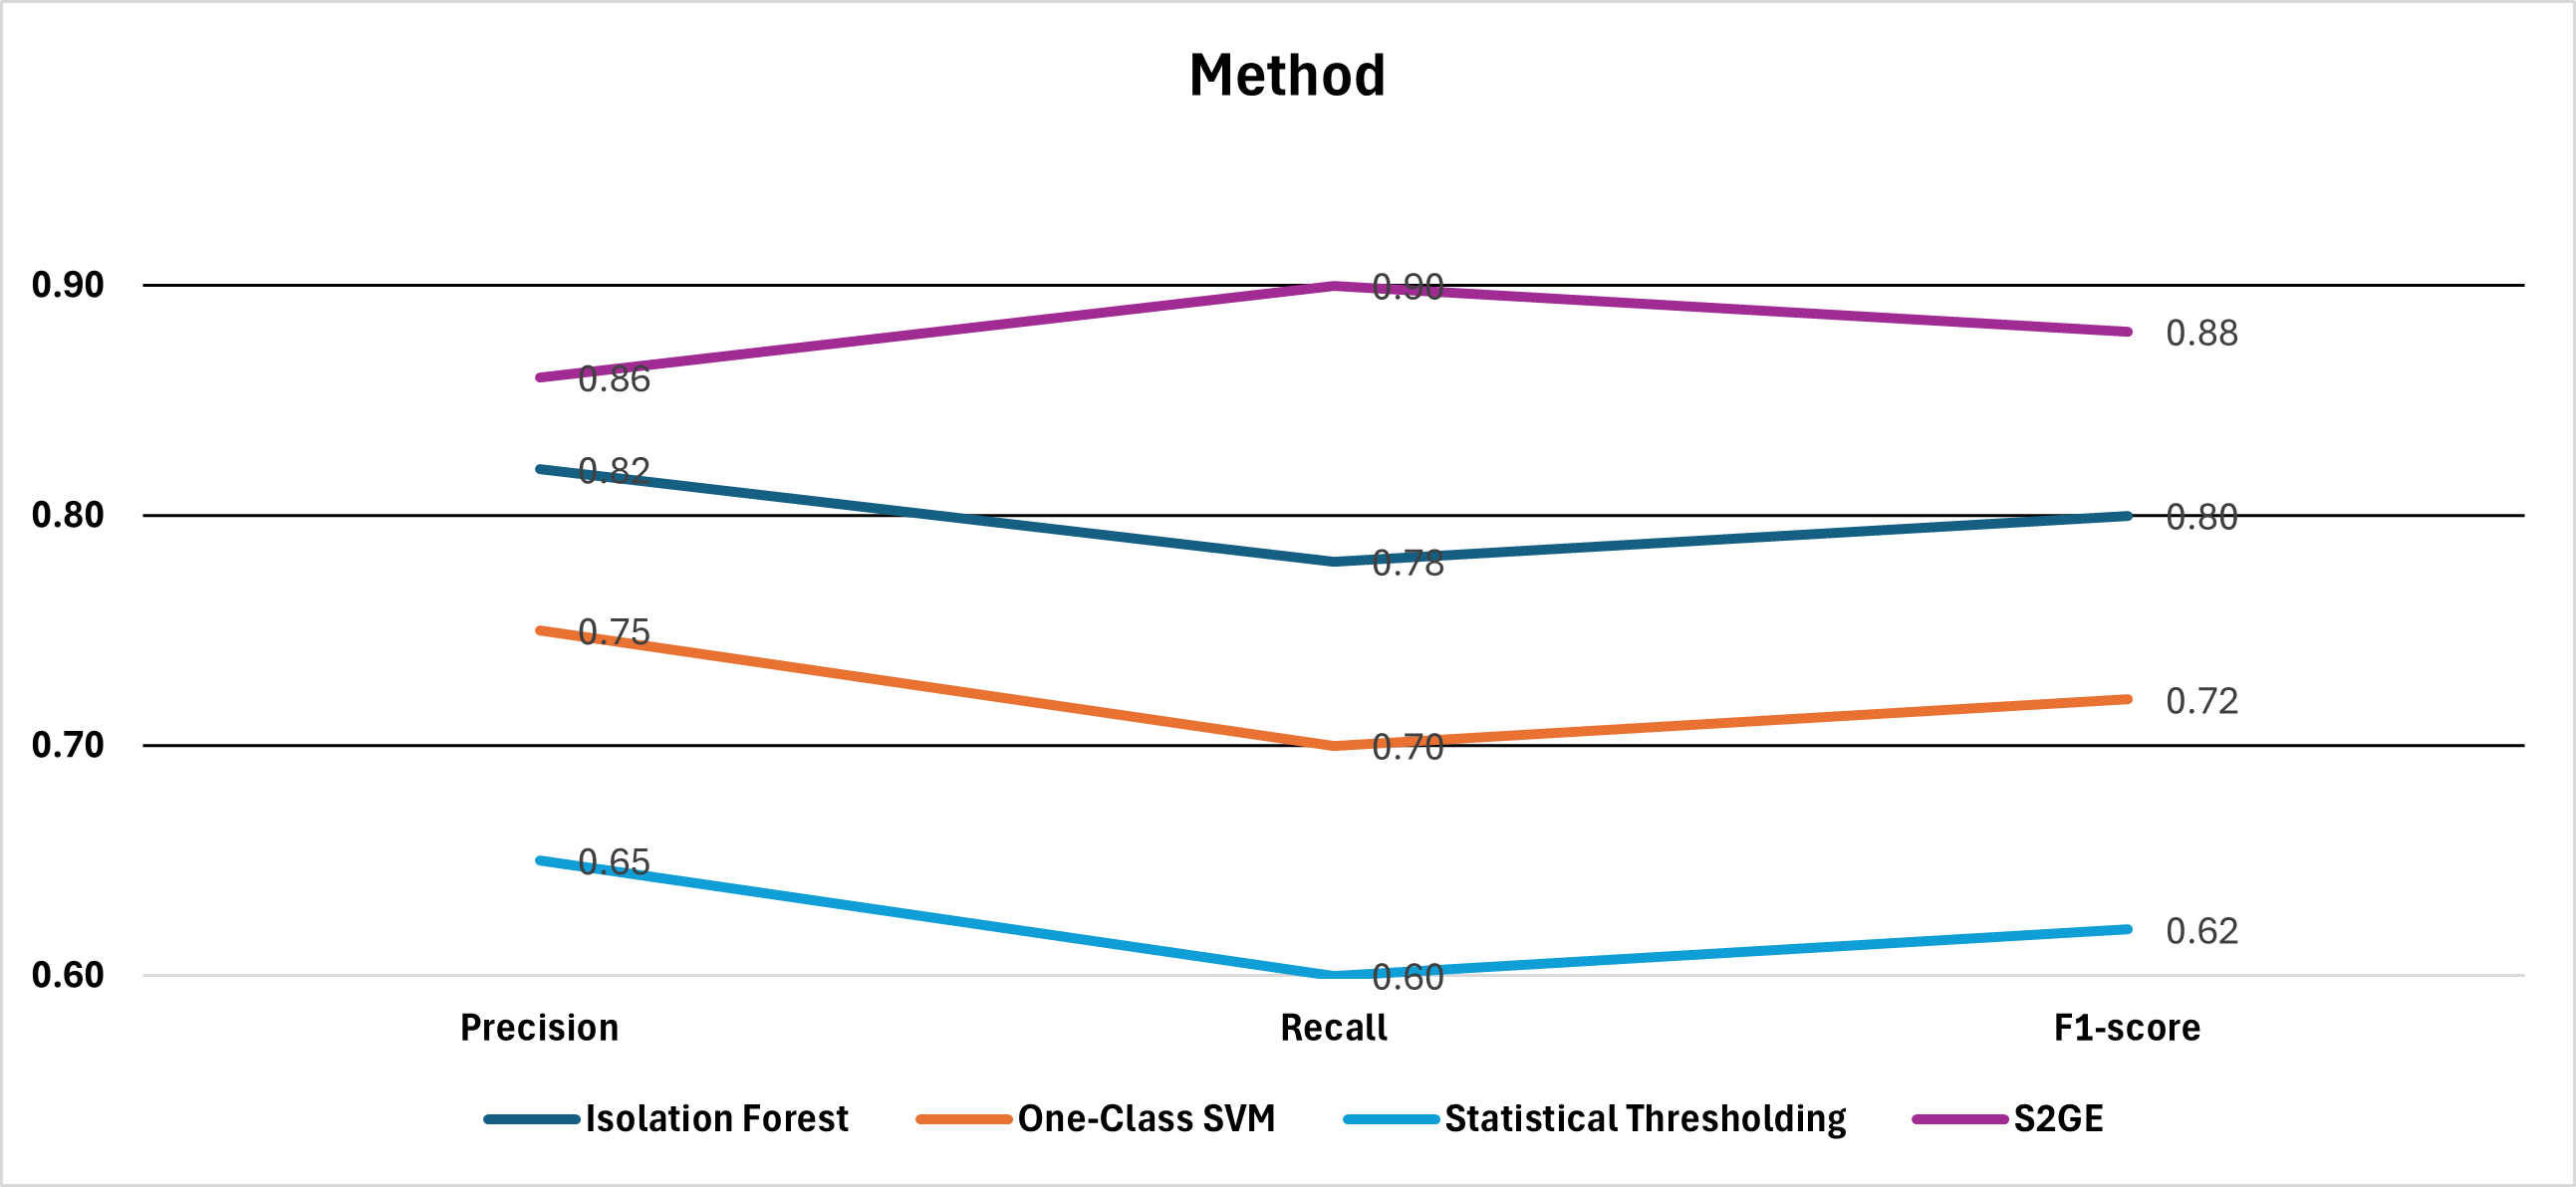
\includegraphics[width = 1\textwidth]{image/Method.png}
        \caption{Mahalanobis Distances and Classification Results of Anomalous Samples}
        \label{fig:method_compare}
    \end{figure*}

    \newpage
    Figure~\ref{fig:method_compare} shows that performance comparison of different anomaly detection methods on Precision, Recall, and F1-score metrics.
    The purple line represents the proposed S2GE method, which achieves the highest scores across all three metrics.
    Isolation Forest (blue) and AutoEncoder (green) demonstrate moderate performance,
    This visualization clearly highlights the superior detection capability of S2GE in terms of both accuracy and recall.




\end{ZhChapter}